\section{Overall description}
\subsection{Product perspective}
\todo{class diagrams, statecharts, communication}
	\subsubsection{System interfaces}
	\label{sec:systemInterfaces}
		The system we are to develop will have some external interfaces (represented in \autoref{fig:systemInterfaces}) to accomplish the \hyperref[sec:goals]{goals stated before}.
		\begin{figure}[h]
			\centering
			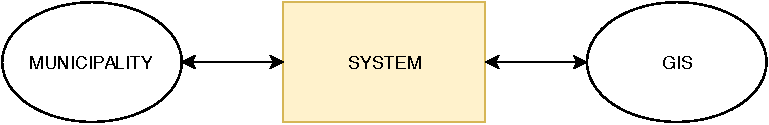
\includegraphics[width=300, height=50]{system_blocks}
			\caption{
				\label{fig:systemInterfaces} 
				Overview of system interfaces
			}
		\end{figure}
	\paragraph{Municipality}
	The system will interact with municipalities. Our system will retrieve the information about the accidents that occur on the territory of the municipality and cross this information with its own data to identify potentially unsafe areas. It will also retrieve the information about issued tickets from the municipalities to build statistics, for example about the most egregious offenders, or the effectiveness of the SafeStreets initiative (e.g., by looking for trends in the issuing of tickets).
	
	 In addition, our system will expose via a \emph{restricted access API} the stored information about the violations to the municipalities, so that the local authorities can generates traffic tickets from it, and suggest possible interventions (e.g., add a barrier between the bike lane and the part of the road for motorized vehicles to prevent unsafe parking). 
	 
	\paragraph{Map} Highlighted streets (or areas) with the highest frequency of violations, and unsafe areas are displayed to all users on an up-to-date map which relies on an external GIS.

\subsubsection{User interfaces}		
\paragraph{Guest user}
	Using the interfaces of the system users can:
	\begin{enumerate}
		\item Register to the system or request an account for a specific municipality
		\item Log-in to the system
	\end{enumerate}
\paragraph{Logged User}
	Using the interfaces of the system users can:
	\begin{enumerate}
		\item Submit a violation with all the required and optional metadata
		\item View a map through an external GIS with highlighted streets (or areas) with the highest frequency of violations
		\item View statistics on vehicles that commit the most violations, the most egregious offenders, or the effectiveness of the SafeStreets initiative.
		\item View and edit personal information
	\end{enumerate}
	
\subsubsection{Software interfaces}
Databases and DBMSs are clearly required in order to store data about users, violations, safe/unsafe areas etc.

As mentioned before (see \hyperref[sec:systemInterfaces]{system interfaces section}) the system needs to use external APIs and to expose interfaces in order to interact with other systems.

\subsection{Product functions}
\todo{}

\subsection{User characteristics}
	Users can use our system when they want to rent a car.\\
	Necessary conditions for the user in order to use the system are:
	\begin{itemize}
		\item He must have a smartphone and be able to use it
		\item He must be in the age of majority
		\item He must have a proper valid driving license
		\item He must be able to drive a car (i.d. he must be in both physical and mental health)
	\end{itemize}
	The user agrees to these conditions during the registration to the system.

\subsection{Domain assumption}
	We assume that these assumptions hold true in the domain of our system 
	\begin{enumerate}[label=\textbf{DA\arabic*}]
		\item GPS position is supposed to be accurate (max error $\pm5$m)
		\item GPS position of all cars is always obtainable
		\item The user who reserves the car will always be the person who drives it
		\item Users are legally allowed to drive cars (i.d. users have a proper driving license)
		\item Charging stations are always working correctly
		\item \label{da:userGivenInfo} All information provided by users are correct and reliable
		\item All cars provided by the customer are equipped with a module which provides a set of
		primitives that allow the system to retrieve all the information it needs about
		the car and to run commands which allow the system to take actions on the car (see \hyperref[sec:cars]{cars section} for more details)
		\item Charging station can exclusively be used by PowerEnJoy cars
		\item The set of safe areas is pre-defined and is provided to our system by the customer
		\item The position of charging station is provided to our system by the customer
		\item All charging station are located inside safe areas
		\item The maps provided by the GIS are always up to date
		\item The commands sent to cars by the system are always executed
		correctly
		\item Information provided by the car are always correct and reliable
		\item Position of the user is always available when he uses our system
		\item \label{da:zeroBattery}Even if the car is left with no battery left, it is still able to communicate with the system
		
	\end{enumerate}
\clearpage